\chapter{Arkitektur}

% Beskrivelse af den overordnede systemarkitektur. Her skal SysML blok diagrammer benyttes. Der gives et overblik over systemets arkitektur med udgangspunkt og reference til jeres systemarkitektur dokument.

I dette afsnit beskrives den overordnede arkitektur for systemet. Systemets arkitektur har dannet ramme for design og senere implementering. Til at beskrive systemets arkitektur bruges 4+1 modellen som kan ses på figur~\ref{fig:41model}. Modellen er udviklet af Philippe Kruchten~\cite{fcgss2007}. Modellen indeholder fire views samt et user-story eller use-cases view.

\begin{itemize}
	\item Logical view - End-user funktionalitet
	\begin{itemize}
		\item Klassediagrammer
		\item Package diagram
		\item State machine diagram
	\end{itemize}
	\item Process view - Adfærd og performance
	\begin{itemize}
		\item Activity diagram
		\item Sekvens diagram
	\end{itemize}
	\item Implementation/Development view - Udviklerperspektivet
	\begin{itemize}
		\item Component diagram
	\end{itemize}
	\item Physical view - Fysiske bindinger i systemet
	\begin{itemize}
		\item Deployment diagram
	\end{itemize}
\end{itemize}

\begin{figure}[h]
	\centering
	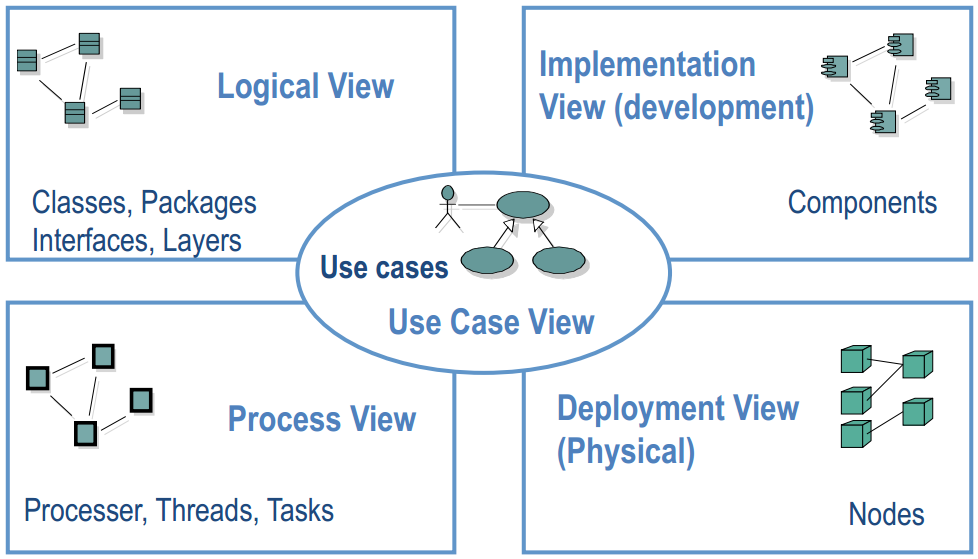
\includegraphics[width=0.8\linewidth]{figs/arkitektur/41model}
	\caption{$4+1$ Arkitektur modellen \cite{flylib}}
	\label{fig:41model}
\end{figure}

\section{Logical view}


\section{Process view}
\todo{Skriv kort om development viewet.}

\section{Implementation/Development view}
\todo{Skriv kort om development viewet.}

På figur \ref{fig:packageDiagram} ses projektets packagediagram.

Package diagrammet har til formål at vise systemets afhængigheder. Disse er vist med en stiplet pil. En fuldoptrukket linje med + betyder "\textit{nested} og altså at pakken er indeholdt i den anden pakke. Pakken \textit{External DLL's} er eksterne afhængigheder, såsom library filer og DLL'er der bruges.

\begin{landscape}
	\begin{figure}[H]
		\centering
		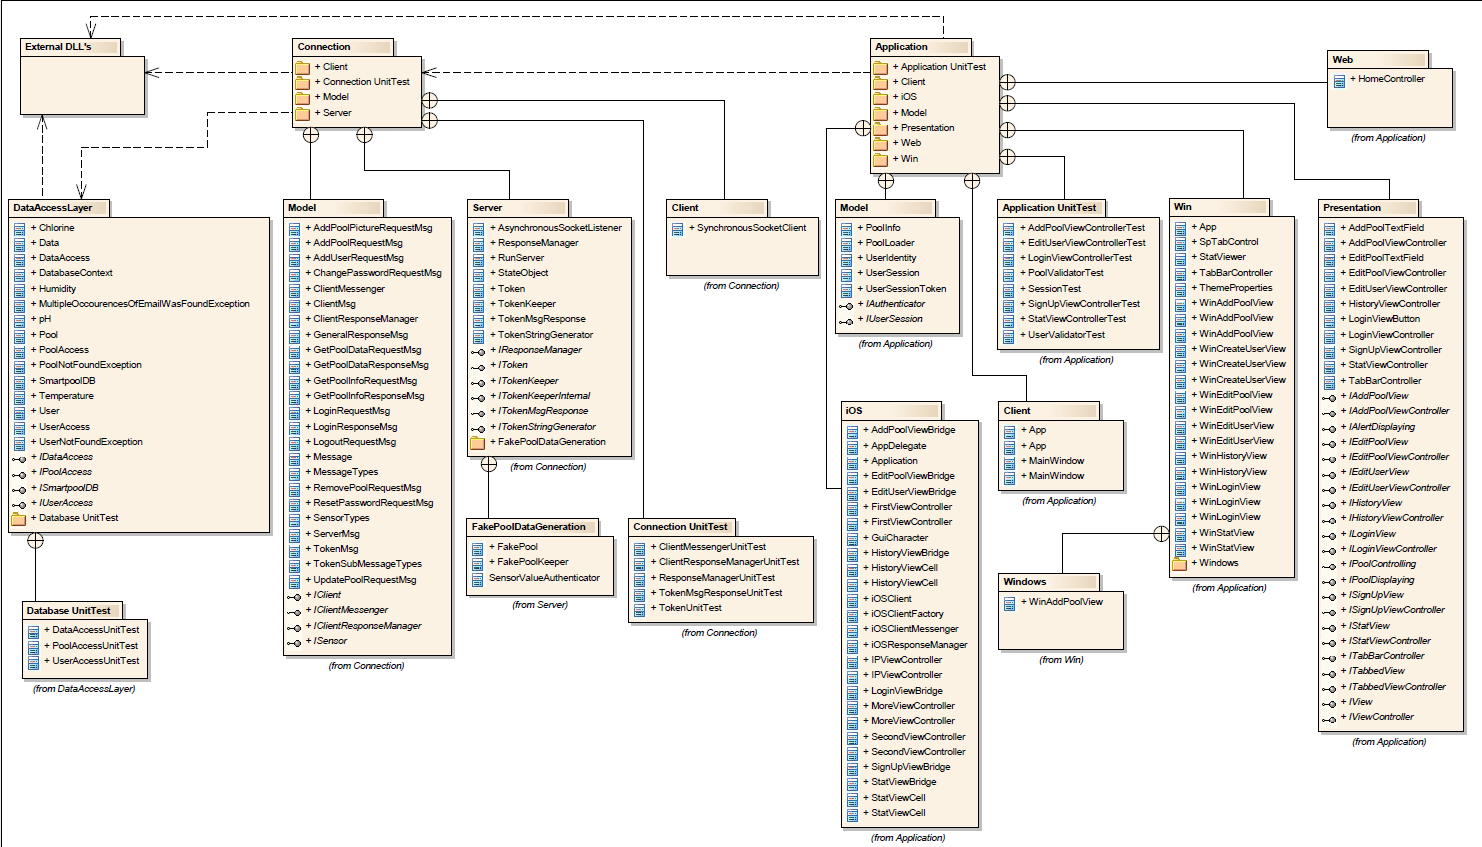
\includegraphics[width=\linewidth]{figs/arkitektur/packageDiagram.PNG}
		\caption{Package model - Implementation/Development view}
		\label{fig:packageDiagram}
	\end{figure}
\end{landscape}

\section{Physical view}
\todo{Skriv kort om development viewet.}
 
Deployment diagrammet har til formål at vise systemets hardware (Klienter, servere og databaser), og hvordan de kommunikerer. Da Smartpool systemet er udviklet til flere typer af kienter, herunder iOS, Windows og Internet browsere giver deployment diagrammet god indsigt i hvordan elementerne hænger sammen.
På figur \ref{fig:deploymentView} ses projektets deployment diagram.

\begin{figure}
	\centering
	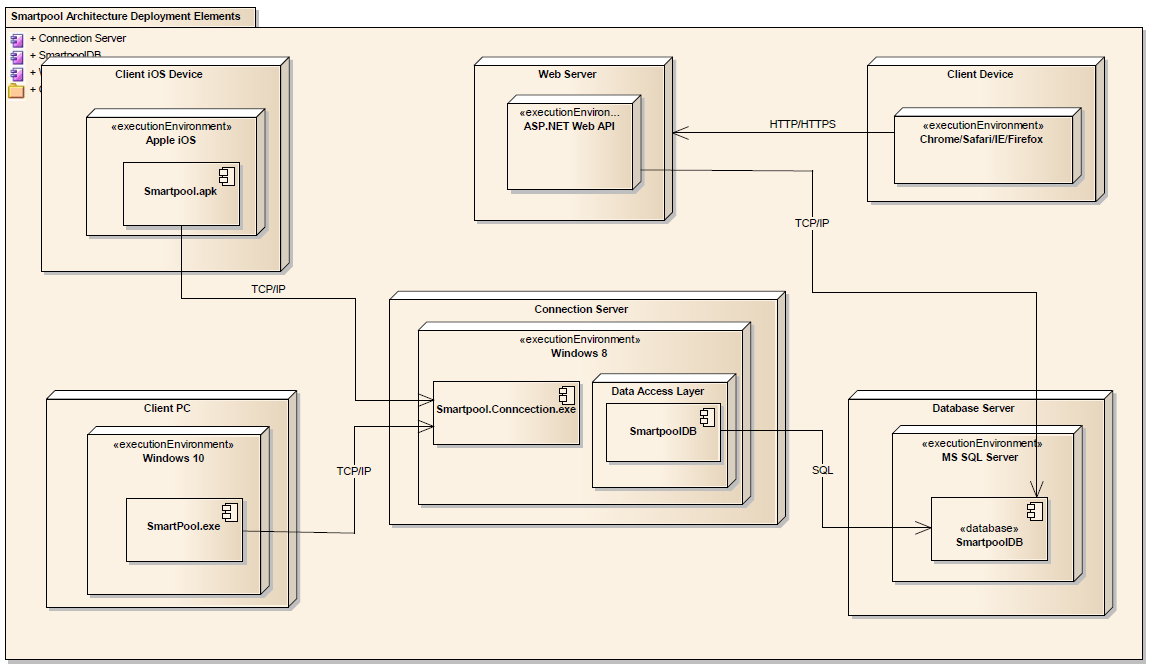
\includegraphics[width=\linewidth]{figs/arkitektur/deploymentView.PNG}
	\caption{Deployment diagram - Physical view}
	\label{fig:deploymentView}
\end{figure}

